\documentclass{standalone}
\usepackage{tikz}
\usetikzlibrary{patterns, positioning}


\begin{document}
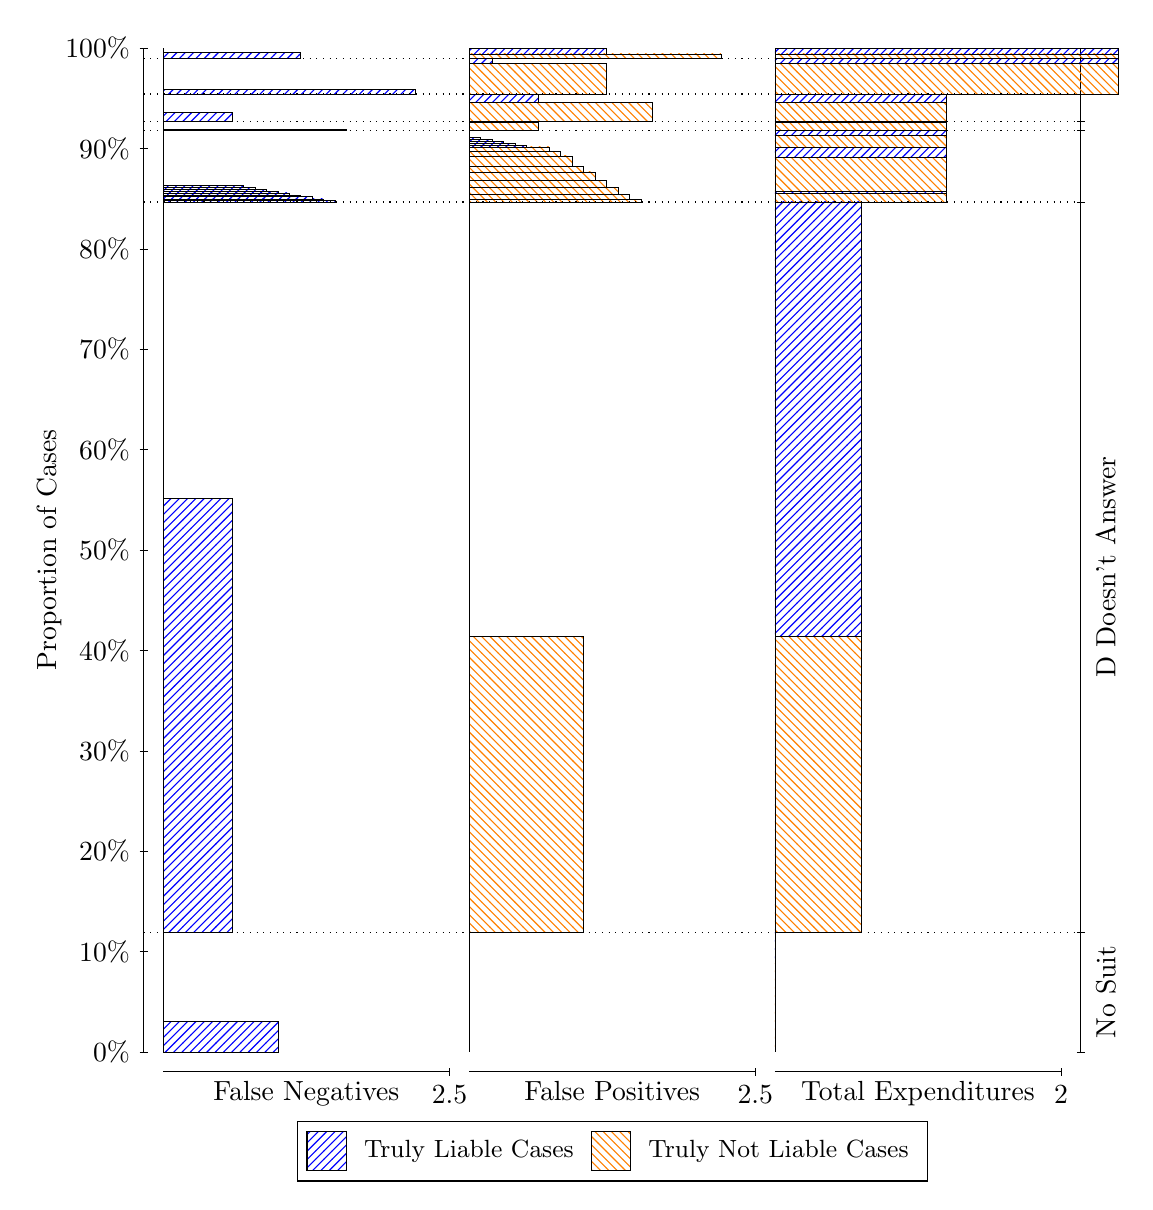
\begin{tikzpicture}
\draw[black, very thin] (1.5,1.75) -- (1.5,14.5);
\node[rotate=90, text=black, anchor=center] at (0.3, 8.125) {Proportion of Cases};
\draw[black, very thin] (1.45,1.75) -- (1.55,1.75);
\node[text=black, anchor=east] at (1.45, 1.75) {0\%};
\draw[black, very thin] (1.45,3.025) -- (1.55,3.025);
\node[text=black, anchor=east] at (1.45, 3.025) {10\%};
\draw[black, very thin] (1.45,4.3) -- (1.55,4.3);
\node[text=black, anchor=east] at (1.45, 4.3) {20\%};
\draw[black, very thin] (1.45,5.575) -- (1.55,5.575);
\node[text=black, anchor=east] at (1.45, 5.575) {30\%};
\draw[black, very thin] (1.45,6.85) -- (1.55,6.85);
\node[text=black, anchor=east] at (1.45, 6.85) {40\%};
\draw[black, very thin] (1.45,8.125) -- (1.55,8.125);
\node[text=black, anchor=east] at (1.45, 8.125) {50\%};
\draw[black, very thin] (1.45,9.4) -- (1.55,9.4);
\node[text=black, anchor=east] at (1.45, 9.4) {60\%};
\draw[black, very thin] (1.45,10.675) -- (1.55,10.675);
\node[text=black, anchor=east] at (1.45, 10.675) {70\%};
\draw[black, very thin] (1.45,11.95) -- (1.55,11.95);
\node[text=black, anchor=east] at (1.45, 11.95) {80\%};
\draw[black, very thin] (1.45,13.225) -- (1.55,13.225);
\node[text=black, anchor=east] at (1.45, 13.225) {90\%};
\draw[black, very thin] (1.45,14.5) -- (1.55,14.5);
\node[text=black, anchor=east] at (1.45, 14.5) {100\%};

\draw[black, very thin] (13.4,1.75) -- (13.4,14.5);
\draw[black, very thin] (13.35,1.75) -- (13.45,1.75);
\node[anchor=west] at (13.35, 1.75) {};
\draw[black, very thin] (13.35,3.2717) -- (13.45,3.2717);
\node[anchor=west] at (13.35, 3.2717) {};
\draw[black, very thin] (13.35,12.545) -- (13.45,12.545);
\node[anchor=west] at (13.35, 12.545) {};
\draw[black, very thin] (13.35,13.45) -- (13.45,13.45);
\node[anchor=west] at (13.35, 13.45) {};
\draw[black, very thin] (13.35,13.569) -- (13.45,13.569);
\node[anchor=west] at (13.35, 13.569) {};
\draw[black, very thin] (13.35,13.916) -- (13.45,13.916);
\node[anchor=west] at (13.35, 13.916) {};
\draw[black, very thin] (13.35,14.366) -- (13.45,14.366);
\node[anchor=west] at (13.35, 14.366) {};
\draw[black, very thin] (13.35,14.5) -- (13.45,14.5);
\node[anchor=west] at (13.35, 14.5) {};

\draw[black, very thin, pattern color=blue, pattern=north east lines] (1.75,1.75) rectangle (3.2033,2.1434);
\draw[black, very thin, pattern color=orange, pattern=north west lines] (1.75,2.1434) rectangle (1.75,3.2717);
\draw[black, very thin, pattern color=blue, pattern=north east lines] (1.75,3.2717) rectangle (2.622,8.7845);
\draw[black, very thin, pattern color=orange, pattern=north west lines] (1.75,8.7845) rectangle (1.75,12.545);
\draw[black, very thin, pattern color=blue, pattern=north east lines] (1.75,12.545) rectangle (3.93,12.565);
\draw[black, very thin, pattern color=blue, pattern=north east lines] (1.75,12.565) rectangle (3.7847,12.583);
\draw[black, very thin, pattern color=blue, pattern=north east lines] (1.75,12.583) rectangle (3.6393,12.613);
\draw[black, very thin, pattern color=blue, pattern=north east lines] (1.75,12.613) rectangle (3.494,12.633);
\draw[black, very thin, pattern color=blue, pattern=north east lines] (1.75,12.633) rectangle (3.3487,12.66);
\draw[black, very thin, pattern color=blue, pattern=north east lines] (1.75,12.66) rectangle (3.2033,12.677);
\draw[black, very thin, pattern color=blue, pattern=north east lines] (1.75,12.677) rectangle (3.058,12.707);
\draw[black, very thin, pattern color=blue, pattern=north east lines] (1.75,12.707) rectangle (2.9127,12.731);
\draw[black, very thin, pattern color=blue, pattern=north east lines] (1.75,12.731) rectangle (2.7673,12.751);
\draw[black, very thin, pattern color=orange, pattern=north west lines] (1.75,12.751) rectangle (1.75,13.45);
\draw[black, very thin, pattern color=blue, pattern=north east lines] (1.75,13.45) rectangle (4.0753,13.468);
\draw[black, very thin, pattern color=orange, pattern=north west lines] (1.75,13.468) rectangle (1.75,13.569);
\draw[black, very thin, pattern color=blue, pattern=north east lines] (1.75,13.569) rectangle (2.622,13.679);
\draw[black, very thin, pattern color=orange, pattern=north west lines] (1.75,13.679) rectangle (1.75,13.916);
\draw[black, very thin, pattern color=blue, pattern=north east lines] (1.75,13.916) rectangle (4.9473,13.977);
\draw[black, very thin, pattern color=orange, pattern=north west lines] (1.75,13.977) rectangle (1.75,14.366);
\draw[black, very thin, pattern color=blue, pattern=north east lines] (1.75,14.366) rectangle (3.494,14.441);
\draw[black, very thin, pattern color=orange, pattern=north west lines] (1.75,14.441) rectangle (1.75,14.5);
\draw[black, very thin, pattern color=orange, pattern=north west lines] (5.6333,1.75) rectangle (5.6333,2.8783);
\draw[black, very thin, pattern color=blue, pattern=north east lines] (5.6333,2.8783) rectangle (5.6333,3.2717);
\draw[black, very thin, pattern color=orange, pattern=north west lines] (5.6333,3.2717) rectangle (7.0867,7.0323);
\draw[black, very thin, pattern color=blue, pattern=north east lines] (5.6333,7.0323) rectangle (5.6333,12.545);
\draw[black, very thin, pattern color=orange, pattern=north west lines] (5.6333,12.545) rectangle (7.8133,12.578);
\draw[black, very thin, pattern color=orange, pattern=north west lines] (5.6333,12.578) rectangle (7.668,12.637);
\draw[black, very thin, pattern color=orange, pattern=north west lines] (5.6333,12.637) rectangle (7.5227,12.734);
\draw[black, very thin, pattern color=orange, pattern=north west lines] (5.6333,12.734) rectangle (7.3773,12.817);
\draw[black, very thin, pattern color=orange, pattern=north west lines] (5.6333,12.817) rectangle (7.232,12.927);
\draw[black, very thin, pattern color=orange, pattern=north west lines] (5.6333,12.927) rectangle (7.0867,13);
\draw[black, very thin, pattern color=orange, pattern=north west lines] (5.6333,13) rectangle (6.9413,13.13);
\draw[black, very thin, pattern color=orange, pattern=north west lines] (5.6333,13.13) rectangle (6.796,13.188);
\draw[black, very thin, pattern color=orange, pattern=north west lines] (5.6333,13.188) rectangle (6.6507,13.244);
\draw[black, very thin, pattern color=blue, pattern=north east lines] (5.6333,13.244) rectangle (6.36,13.264);
\draw[black, very thin, pattern color=blue, pattern=north east lines] (5.6333,13.264) rectangle (6.2147,13.288);
\draw[black, very thin, pattern color=blue, pattern=north east lines] (5.6333,13.288) rectangle (6.0693,13.318);
\draw[black, very thin, pattern color=blue, pattern=north east lines] (5.6333,13.318) rectangle (5.924,13.335);
\draw[black, very thin, pattern color=blue, pattern=north east lines] (5.6333,13.335) rectangle (5.7787,13.362);
\draw[black, very thin, pattern color=blue, pattern=north east lines] (5.6333,13.362) rectangle (5.6333,13.45);
\draw[black, very thin, pattern color=orange, pattern=north west lines] (5.6333,13.45) rectangle (6.5053,13.551);
\draw[black, very thin, pattern color=blue, pattern=north east lines] (5.6333,13.551) rectangle (5.6333,13.569);
\draw[black, very thin, pattern color=orange, pattern=north west lines] (5.6333,13.569) rectangle (7.9587,13.806);
\draw[black, very thin, pattern color=blue, pattern=north east lines] (5.6333,13.806) rectangle (6.5053,13.916);
\draw[black, very thin, pattern color=orange, pattern=north west lines] (5.6333,13.916) rectangle (7.3773,14.305);
\draw[black, very thin, pattern color=blue, pattern=north east lines] (5.6333,14.305) rectangle (5.924,14.366);
\draw[black, very thin, pattern color=orange, pattern=north west lines] (5.6333,14.366) rectangle (8.8307,14.426);
\draw[black, very thin, pattern color=blue, pattern=north east lines] (5.6333,14.426) rectangle (7.3773,14.5);
\draw[black, very thin, pattern color=orange, pattern=north west lines] (9.5167,1.75) rectangle (9.5167,2.8783);
\draw[black, very thin, pattern color=blue, pattern=north east lines] (9.5167,2.8783) rectangle (9.5167,3.2717);
\draw[black, very thin, pattern color=orange, pattern=north west lines] (9.5167,3.2717) rectangle (10.607,7.0323);
\draw[black, very thin, pattern color=blue, pattern=north east lines] (9.5167,7.0323) rectangle (10.607,12.545);
\draw[black, very thin, pattern color=orange, pattern=north west lines] (9.5167,12.545) rectangle (11.697,12.655);
\draw[black, very thin, pattern color=blue, pattern=north east lines] (9.5167,12.655) rectangle (11.697,12.682);
\draw[black, very thin, pattern color=orange, pattern=north west lines] (9.5167,12.682) rectangle (11.697,13.115);
\draw[black, very thin, pattern color=blue, pattern=north east lines] (9.5167,13.115) rectangle (11.697,13.239);
\draw[black, very thin, pattern color=orange, pattern=north west lines] (9.5167,13.239) rectangle (11.697,13.395);
\draw[black, very thin, pattern color=blue, pattern=north east lines] (9.5167,13.395) rectangle (11.697,13.45);
\draw[black, very thin, pattern color=orange, pattern=north west lines] (9.5167,13.45) rectangle (11.697,13.551);
\draw[black, very thin, pattern color=blue, pattern=north east lines] (9.5167,13.551) rectangle (11.697,13.569);
\draw[black, very thin, pattern color=orange, pattern=north west lines] (9.5167,13.569) rectangle (11.697,13.806);
\draw[black, very thin, pattern color=blue, pattern=north east lines] (9.5167,13.806) rectangle (11.697,13.916);
\draw[black, very thin, pattern color=orange, pattern=north west lines] (9.5167,13.916) rectangle (13.877,14.305);
\draw[black, very thin, pattern color=blue, pattern=north east lines] (9.5167,14.305) rectangle (13.877,14.366);
\draw[black, very thin, pattern color=orange, pattern=north west lines] (9.5167,14.366) rectangle (13.877,14.426);
\draw[black, very thin, pattern color=blue, pattern=north east lines] (9.5167,14.426) rectangle (13.877,14.5);
\draw[black, dotted] (1.5,3.2717) -- (13.4,3.2717);
\draw[black, dotted] (1.5,12.545) -- (13.4,12.545);
\draw[black, dotted] (1.5,13.45) -- (13.4,13.45);
\draw[black, dotted] (1.5,13.569) -- (13.4,13.569);
\draw[black, dotted] (1.5,13.916) -- (13.4,13.916);
\draw[black, dotted] (1.5,14.366) -- (13.4,14.366);
\draw[black, very thin] (1.75,1.5) -- (5.3833,1.5);
\node[text=black, anchor=north] at (3.5667, 1.5) {False Negatives};
\draw[black, very thin] (5.3833,1.45) -- (5.3833,1.55);
\node[text=black, anchor=north] at (5.3833, 1.45) {2.5};

\draw[black, very thin] (5.6333,1.5) -- (9.2667,1.5);
\node[text=black, anchor=north] at (7.45, 1.5) {False Positives};
\draw[black, very thin] (9.2667,1.45) -- (9.2667,1.55);
\node[text=black, anchor=north] at (9.2667, 1.45) {2.5};

\draw[black, very thin] (9.5167,1.5) -- (13.15,1.5);
\node[text=black, anchor=north] at (11.333, 1.5) {Total Expenditures};
\draw[black, very thin] (13.15,1.45) -- (13.15,1.55);
\node[text=black, anchor=north] at (13.15, 1.45) {2};

\node[text=black, centered, rotate=90] at (13.72, 2.5109) {No Suit};
\node[text=black, centered, rotate=90] at (13.72, 7.9084) {D Doesn't Answer};






\draw (7.449999999999999,1.5) node[draw=none] (baseCoordinate) {};
\begin{scope}[align=center]
        \matrix[scale=0.5, draw=black, below=0.5cm of baseCoordinate, nodes={draw}, column sep=0.1cm]{
            \node[rectangle, draw, minimum width=0.5cm, minimum height=0.5cm, pattern color=blue, pattern=north east lines] {}; &
            \node[draw=none, font=\small, text=black] (B) {Truly Liable Cases}; &
            \node[rectangle, draw, minimum width=0.5cm, minimum height=0.5cm, pattern color=orange, pattern=north west lines] {}; &
            \node[draw=none, font=\small, text=black] (B) {Truly Not Liable Cases}; \\
            };
\end{scope}

\end{tikzpicture}
\end{document}